\chapter{Giới Thiệu Đề Tài}

\section{Đặt vấn đề}
Trong những năm gần đây, ô nhiễm không khí tại các đô thị lớn ở Việt Nam, đặc biệt là Hà Nội, đã trở thành một thách thức lớn đối với sức khỏe cộng đồng. Theo các báo cáo quan trắc môi trường, nồng độ bụi mịn PM2.5, PM10 và các khí độc hại từ khí thải phương tiện giao thông thường xuyên vượt ngưỡng an toàn cho phép của Tổ chức Y tế Thế giới (WHO). Tác hại của ô nhiễm không khí ảnh hưởng trực tiếp đến hệ hô hấp, tim mạch và làm giảm chất lượng cuộc sống của người dân.

Trong khi các trạm quan trắc không khí chuyên nghiệp của nhà nước cung cấp dữ liệu có độ chính xác cao, số lượng trạm đo lại rất hạn chế và khoảng cách giữa các trạm quá lớn. Điều này dẫn đến việc dữ liệu đo đạc không phản ánh được mức độ ô nhiễm cục bộ trong các không gian nhỏ như: phòng học, phòng thí nghiệm, văn phòng làm việc hay khu vực đỗ xe (nhà gửi xe). Đặc biệt, khu vực nhà gửi xe là nơi thường xuyên tích tụ nồng độ khí thải độc hại (CO, CO2, VOCs) và bụi mịn phát ra từ động cơ phương tiện giao thông khi khởi động. Do đó, việc xây dựng các trạm quan trắc không khí cục bộ chi phí thấp, hoạt động ổn định và có khả năng cảnh báo kịp thời là vô cùng cần thiết.

Tuy nhiên, các giải pháp đo chất lượng không khí tự chế (DIY/IoT) trên thị trường hiện nay thường gặp phải hai nhược điểm lớn:
\begin{enumerate}
    \item \textbf{Độ ổn định của luồng khí lấy mẫu}: Cảm biến bụi và cảm biến khí đặt tự do ngoài không khí thường bị ảnh hưởng bởi hướng gió không kiểm soát hoặc nhiệt độ cục bộ do linh kiện tỏa ra, gây sai số phép đo.
    \item \textbf{Mất dữ liệu khi mất kết nối mạng}: Các thiết bị IoT thường gửi dữ liệu trực tiếp lên cloud. Khi mất kết nối Wi-Fi hoặc máy chủ gặp sự cố, dữ liệu đo đạc trong khoảng thời gian đó sẽ bị mất hoàn toàn, gây gián đoạn việc ghi lại số liệu lịch sử trong khoảng thời gian thiết bị hoạt động.
\end{enumerate}

Xuất phát từ thực tiễn trên, đề tài \textbf{"Nâng cấp hệ thống đo và cảnh báo chất lượng không khí sử dụng vi điều khiển ESP32"} được lựa chọn nhằm giải quyết các bài toán trên thông qua việc thiết kế buồng lấy mẫu khí chủ động, tích hợp cơ chế lưu trữ ngoại tuyến tạm thời (offline caching) và hệ thống cảnh báo từ xa đa kênh.
\newpage
\section{Mục tiêu và phạm vi đề tài}
\subsection{Mục tiêu đề tài}
Mục tiêu tổng quát của đề tài là nghiên cứu, thiết kế và chế tạo một nguyên mẫu hệ thống đo chất lượng không khí cục bộ có thể hoạt động ổn định, độ tin cậy ở múc trung bình tới khá cao và chi phí thấp. Cụ thể, hệ thống cần đạt được các mục tiêu kỹ thuật sau:
\begin{itemize}
    \item Thu thập chính xác theo thời gian thực các chỉ số môi trường gồm: nhiệt độ, độ ẩm, nồng độ khí gas tổng quát (MQ135), nồng độ bụi mịn tương đối (GP2Y1010AU0F), áp suất khí quyển.
    \item Cải tiến cấu trúc phần cứng bằng cách thiết kế buồng đo khí chủ động có quạt hút lấy mẫu khí định lượng để bảo vệ cảm biến khỏi tác động trực tiếp của môi trường bên ngoài và giảm nhiệt độ cục bộ.
    \item Xây dựng firmware đa tác vụ trên nền tảng FreeRTOS để quản lý tối ưu tài nguyên vi điều khiển ESP32, đảm bảo hệ thống hoạt động non-blocking.
    \item Phát triển cơ chế lưu trữ dữ liệu dự phòng offline (offline caching) trên bộ nhớ flash nội bộ (SPIFFS) để lưu trữ tạm thời các bản ghi khi mất mạng và tự động đồng bộ bù lên cloud khi có kết nối trở lại.
    \item Tích hợp dịch vụ đám mây Supabase để lưu trữ dữ liệu lịch sử lâu dài và cấu hình hệ thống Edge Functions kết hợp Telegram Bot phát tín hiệu cảnh báo từ xa tự động.
    \item Triển khai thực nghiệm đo đạc kéo dài và thực hiện phân tích hiệu chuẩn cảm biến bằng các thuật toán học máy (Machine Learning) để kiểm chứng và đánh giá sai số cảm biến thô dưới ảnh hưởng của độ ẩm.
\end{itemize}

\subsection{Phạm vi đề tài}
Đề tài tập trung vào việc nghiên cứu và xây dựng một nút đo (node) chất lượng không khí cục bộ đặt tại phòng học hoặc nhà xe. Hệ thống sử dụng các cảm biến bán dẫn và quang học giá rẻ. Kết quả đo đạc từ hệ thống mang tính chất tham khảo, giúp nhận biết xu hướng biến thiên của môi trường và đưa ra cảnh báo sớm, không nhằm thay thế các thiết bị đo kiểm chuẩn của cơ quan khí tượng thủy văn quốc gia.

\section{Định hướng giải pháp}
Để đạt được các mục tiêu đề ra, nhóm thực hiện đề xuất định hướng giải pháp tích hợp phần cứng và phần mềm như sau:

\begin{figure}[H]
    \centering
    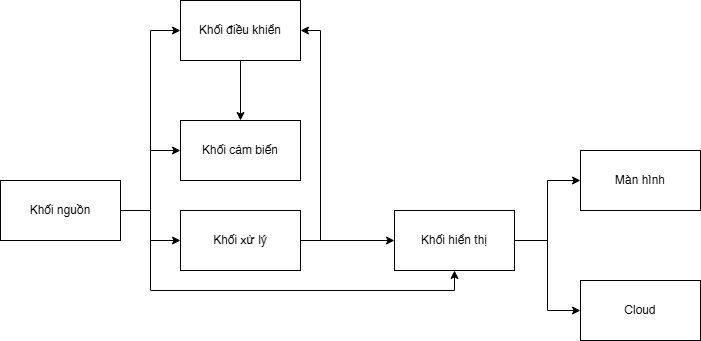
\includegraphics[
        width=0.95\textwidth,
        height=0.45\textheight,
        keepaspectratio
    ]{images/so_do_khoi_tong_quan.png}
    \caption{Định hướng giải pháp kiến trúc hệ thống}
    \label{fig:overviewsolution}
\end{figure}

\begin{itemize}
    \item \textbf{Về phần cứng}: Sử dụng chip SoC ESP32-WROOM-32 làm bộ xử lý trung tâm. Thiết kế bo mạch mạch in (PCB) tích hợp đầy đủ khối nguồn bảo vệ sụt áp, các mạch đệm điều khiển quạt hút 5V và còi buzzer cảnh báo qua relay 5V 1 kênh.
    \item \textbf{Về firmware}: Lập trình C++ trên công cụ PlatformIO. Tổ chức mã nguồn thành các task chạy song song trên FreeRTOS được điều phối đồng bộ qua các khóa Mutex.
    \item \textbf{Về hệ thống đám mây}: Sử dụng cơ sở dữ liệu Postgres của Supabase. Cài đặt các cơ chế Database Webhook và Cron Job phía Server kết hợp với Deno Edge Functions để kiểm tra trạng thái thiết bị trực tuyến (watchdog) và gửi thông tin cảnh báo thông qua Telegram API một cách độc lập, bảo mật.
\end{itemize}

\section{Bố cục báo cáo}
Nội dung báo cáo bài tập lớn được tổ chức thành 6 chương chính và phần phụ lục đi kèm:
\begin{itemize}
    \item \textbf{Chương 1. Giới thiệu đề tài}: Trình bày tính cấp thiết, mục tiêu, phạm vi nghiên cứu và phân công nhiệm vụ trong nhóm.
    \item \textbf{Chương 2. Khảo sát và phân tích yêu cầu}: Khảo sát nhu cầu người dùng, phân tích các giải pháp hiện có, so sánh giao thức và đưa ra các yêu cầu chức năng, phi chức năng.
    \item \textbf{Chương 3. Nền tảng lý thuyết và công nghệ sử dụng}: Trình bày nguyên lý hoạt động của vi điều khiển, các cảm biến, hệ điều hành FreeRTOS, cơ sở dữ liệu đám mây Supabase và hệ thống Edge Functions.
    \item \textbf{Chương 4. Phân tích, thiết kế và đánh giá hệ thống}: Chi tiết hóa sơ đồ nguyên lý phần cứng, thiết kế mạch in PCB, lưu đồ thuật toán firmware, kết quả kiểm thử và xử lý số liệu thực nghiệm bằng thuật toán học máy.
    \item \textbf{Chương 5. Các giải pháp và đóng góp nổi bật}: Đánh giá các điểm cải tiến cốt lõi của đề tài về phần cứng buồng đo, firmware FreeRTOS, SPIFFS offline cache và hệ thống cloud-side alert bảo mật.
    \item \textbf{Chương 6. Kết luận và hướng phát triển}: Đánh giá mức độ hoàn thành chỉ tiêu, tóm tắt hạn chế và đề xuất các giải pháp nâng cấp trong tương lai.
\end{itemize}

\section{Phân công nhiệm vụ}
Để đảm bảo tiến độ triển khai dự án, công việc thiết kế và chế tạo được phân chia chi tiết cho các thành viên trong nhóm dựa trên nhật ký công tác tuần. Bảng phân công nhiệm vụ cụ thể được mô tả trong Bảng \ref{tab:taskallocation}.

\begin{table}[H]
\centering
\caption{Bảng phân công nhiệm vụ và mức độ hoàn thành công việc}
\label{tab:taskallocation}
\small
\renewcommand{\arraystretch}{1.35}
\setlength{\tabcolsep}{6pt}

\begin{tabularx}{\textwidth}{|c|p{3.2cm}|X|c|}
\hline
\textbf{STT} & \textbf{Thành viên} & \textbf{Nhiệm vụ chính được giao} & \textbf{Hoàn thành} \\
\hline

1 & \textbf{Đỗ Đức Huy} &
\begin{itemize}[leftmargin=*, nosep]
    \item Lập trình firmware điều khiển ESP32 trên nền tảng PlatformIO.
    \item Thiết kế cấu trúc firmware đa tác vụ với FreeRTOS gồm \texttt{TaskSensors}, \texttt{TaskOLED} và \texttt{TaskNetwork}.
    \item Cài đặt cơ chế bảo vệ dữ liệu dùng chung bằng Mutex.
    \item Xây dựng chức năng gửi dữ liệu lên Supabase thông qua HTTP POST REST API.
    \item Thiết kế cơ chế lưu trữ ngoại tuyến bằng SPIFFS khi mất kết nối Wi-Fi.
\end{itemize}
& 100\% \\
\hline

2 & \textbf{Trương Việt Anh} &
\begin{itemize}[leftmargin=*, nosep]
    \item Thiết kế sơ đồ nguyên lý và bố trí mạch in PCB trên Altium Designer.
    \item Kiểm tra kết nối phần cứng giữa ESP32, DHT22, MQ135, GP2Y1010AU0F, OLED, LED, buzzer và relay.
    \item Thiết kế khối nguồn 5V và mạch điều khiển tải cho quạt lấy mẫu khí.
    \item Lắp ráp nguyên mẫu phần cứng, kiểm tra dây nối và bố trí các module trong mô hình.
    \item Hỗ trợ kiểm tra buồng lấy mẫu khí và hoạt động của quạt hút.
\end{itemize}
& 100\% \\
\hline

3 & \textbf{Đặng Thái Sơn} &
\begin{itemize}[leftmargin=*, nosep]
    \item Xây dựng kế hoạch kiểm thử hệ thống và bảng test case cho từng module.
    \item Thực hiện kiểm thử các khối cảm biến, hiển thị, cảnh báo, truyền dữ liệu và lưu cache.
    \item Ghi nhận kết quả chạy thử, tổng hợp lỗi phát sinh và đề xuất hướng xử lý.
    \item Hỗ trợ thu thập dữ liệu thực nghiệm từ Serial Monitor hoặc Supabase.
    \item Tổng hợp tài liệu, hình ảnh, nhật ký kỹ thuật và nội dung báo cáo.
\end{itemize}
& 100\% \\
\hline

\end{tabularx}
\end{table}
